\let\negmedspace\undefined
\let\negthickspace\undefined
\documentclass[journal,12pt,onecolumn]{IEEEtran}
\usepackage{cite}
\usepackage{amsmath,amssymb,amsfonts,amsthm}
\usepackage{algorithmic}
\usepackage{graphicx}
\usepackage{textcomp}
\usepackage{xcolor}
\usepackage{txfonts}
\usepackage{listings}
\usepackage{enumitem}
\usepackage{mathtools}
\usepackage{gensymb}
\usepackage{circuitikz}
\usepackage{tkz-euclide} % loads  TikZ and tkz-base
\usepackage{listings}
\usepackage{float}

\newtheorem{theorem}{Theorem}[section]
\newtheorem{problem}{Problem}
\newtheorem{proposition}{Proposition}[section]
\newtheorem{lemma}{Lemma}[section]
\newtheorem{corollary}[theorem]{Corollary}
\newtheorem{example}{Example}[section]
\newtheorem{definition}[problem]{Definition}
%\newtheorem{thm}{Theorem}[section] 
%\newtheorem{defn}[thm]{Definition}
%\newtheorem{algorithm}{Algorithm}[section]
%\newtheorem{cor}{Corollary}
\newcommand{\BEQA}{\begin{eqnarray}}
\newcommand{\EEQA}{\end{eqnarray}}
\newcommand{\system}[1]{\stackrel{#1}{\rightarrow}}

\newcommand{\define}{\stackrel{\triangle}{=}}
\theoremstyle{remark}
\newtheorem{rem}{Remark}
%\bibliographystyle{ieeetr}
\begin{document}
%
\providecommand{\pr}[1]{\ensuremath{\Pr\left(#1\right)}}
\providecommand{\prt}[2]{\ensuremath{p_{#1}^{\left(#2\right)} }}       
\providecommand{\qfunc}[1]{\ensuremath{Q\left(#1\right)}}
\providecommand{\sbrak}[1]{\ensuremath{{}\left[#1\right]}}
\providecommand{\lsbrak}[1]{\ensuremath{{}\left[#1\right.}}
\providecommand{\rsbrak}[1]{\ensuremath{{}\left.#1\right]}}
\providecommand{\brak}[1]{\ensuremath{\left(#1\right)}}
\providecommand{\lbrak}[1]{\ensuremath{\left(#1\right.}}
\providecommand{\rbrak}[1]{\ensuremath{\left.#1\right)}}
\providecommand{\cbrak}[1]{\ensuremath{\left\{#1\right\}}}
\providecommand{\lcbrak}[1]{\ensuremath{\left\{#1\right.}}
\providecommand{\rcbrak}[1]{\ensuremath{\left.#1\right\}}}
\newcommand{\sgn}{\mathop{\mathrm{sgn}}}
\providecommand{\abs}[1]{\left\vert#1\right\vert}
\providecommand{\res}[1]{\Res\displaylimits_{#1}} 
\providecommand{\norm}[1]{\left\lVert#1\right\rVert}
%\providecommand{\norm}[1]{\lVert#1\rVert}
\providecommand{\mtx}[1]{\mathbf{#1}}
\providecommand{\mean}[1]{E\left[ #1 \right]}
\providecommand{\cond}[2]{#1\middle|#2}
\providecommand{\fourier}{\overset{\mathcal{F}}{ \rightleftharpoons}}
\newenvironment{amatrix}[1]{%
  \left(\begin{array}{@{}*{#1}{c}|c@{}}
}{%
  \end{array}\right)
}
%\providecommand{\hilbert}{\overset{\mathcal{H}}{ \rightleftharpoons}}
%\providecommand{\system}{\overset{\mathcal{H}}{ \longleftrightarrow}}
    %\newcommand{\solution}[2]{\textbf{Solution:}{#1}}
\newcommand{\solution}{\noindent \textbf{Solution: }}
\newcommand{\cosec}{\,\text{cosec}\,}
\providecommand{\dec}[2]{\ensuremath{\overset{#1}{\underset{#2}{\gtrless}}}}
\newcommand{\myvec}[1]{\ensuremath{\begin{pmatrix}#1\end{pmatrix}}}
\newcommand{\mydet}[1]{\ensuremath{\begin{vmatrix}#1\end{vmatrix}}}
\newcommand{\myaugvec}[2]{\ensuremath{\begin{amatrix}{#1}#2\end{amatrix}}}
\providecommand{\rank}{\text{rank}}
\providecommand{\pr}[1]{\ensuremath{\Pr\left(#1\right)}}
\providecommand{\qfunc}[1]{\ensuremath{Q\left(#1\right)}}
    \newcommand*{\permcomb}[4][0mu]{{{}^{#3}\mkern#1#2_{#4}}}
\newcommand*{\perm}[1][-3mu]{\permcomb[#1]{P}}
\newcommand*{\comb}[1][-1mu]{\permcomb[#1]{C}}
\providecommand{\qfunc}[1]{\ensuremath{Q\left(#1\right)}}
\providecommand{\gauss}[2]{\mathcal{N}\ensuremath{\left(#1,#2\right)}}
\providecommand{\diff}[2]{\ensuremath{\frac{d{#1}}{d{#2}}}}
\providecommand{\myceil}[1]{\left \lceil #1 \right \rceil }
\newcommand\figref{Fig.~\ref}
\newcommand\tabref{Table~\ref}
\newcommand{\sinc}{\,\text{sinc}\,}
\newcommand{\rect}{\,\text{rect}\,}
%%
%   %\newcommand{\solution}[2]{\textbf{Solution:}{#1}}
%\newcommand{\solution}{\noindent \textbf{Solution: }}
%\newcommand{\cosec}{\,\text{cosec}\,}
%\numberwithin{equation}{section}
%\numberwithin{equation}{subsection}
%\numberwithin{problem}{section}
%\numberwithin{definition}{section}
%\makeatletter
%\@addtoreset{figure}{problem}
%\makeatother

%\let\StandardTheFigure\thefigure
\let\vec\mathbf


\bibliographystyle{IEEEtran}
\title{Gate 2022 EE 25}
\author{HIBA MUHAMMED\\
        EE23BTECH11026}
\maketitle

\section*{Problem Statement}
For the circuit shown below with ideal diodes, the output will be :\\
\brak{A} $V_{\text{out}} = V_{\text{in}} \text{ for } V_{\text{in}}>0 $ \\
\brak{B} $V_{\text{out}} = V_{\text{in}} \text{ for } V_{\text{in}}<0 $ \\
\brak{C} $V_{\text{out}} = -V_{\text{in}} \text{ for } V_{\text{in}}>0 $ \\
\brak{D} $V_{\text{out}} = -V_{\text{in}} \text{ for } V_{\text{in}}<0 $ \\

\begin{figure}[ht]
  \centering
  \resizebox{0.55\columnwidth}{!}{\begin{circuitikz}
\tikzstyle{every node}=[font=\large]
\draw [, line width=0.5pt](6.25,13.75) to[D,l={ \large $D1$}] (9,13.75);
\draw [, line width=0.5pt](9,13.75) to[short, -o] (14.25,13.75);
\draw [, line width=0.5pt](6.25,13.75) to[short, -o] (5.25,13.75);
\draw [, line width=0.5pt](11.75,13.75) to[R] (11.75,10.5);
\draw [, line width=0.5pt](8.5,10.5) to[short, -o] (14.25,10.5);
\draw [, line width=0.5pt](8.5,10.5) to[D,l={ \large $D2$}] (7.25,10.5);
\draw [, line width=0.5pt](7.25,10.5) to[short, -o] (5.25,10.5);
\node [font=\large] at (4.75,12.5) {Vin};
\node [font=\large] at (14.25,12.25) {Vout};
\node [font=\large] at (4.75,13.75) {+};
\node [font=\large] at (14.75,13.75) {+};
\node [font=\large] at (4.75,10.5) {-};
\node [font=\large] at (14.5,10.5) {-};
\end{circuitikz}
}
  \caption{Gate EE 25 fig-1}
  \label{fig:gate_ee_25_1}
\end{figure}

\section*{Solution}

\begin{figure}[H]
  \centering
  \resizebox{0.55\columnwidth}{!}{\begin{circuitikz}
\tikzstyle{every node}=[font=\normalsize]
\draw [](5.75,15) to[short, -o] (3.75,15);
\draw [](5.75,15) to[short, -o] (6.25,15);
\draw [](6.25,15) to[short, -o] (5.75,15);
\draw [](6.25,15) to[short, -o] (13.25,15);
\draw (11,15) to[R] (11,12);
\draw [](11,12) to[short, -o] (13.5,12);
\draw [](11,12) to[short, -o] (3.75,12);
\draw [](5.5,12) to[short, -o] (6.5,12);
\node [font=\normalsize] at (6,15.5) {D1};
\node [font=\normalsize] at (6,11.75) {D2};
\draw [](6.25,12) to[short, -o] (5.75,12);
\node [font=\normalsize] at (11.5,13.5) {R};
\node [font=\normalsize] at (3.75,13.5) {Vi};
\node [font=\normalsize] at (13.5,13.5) {Vo};
\draw[<-, thick] (6.75,14) arc (90:-90:0.5) node[midway, left] {$$};;
\end{circuitikz}
}
  \caption{Gate EE fig-2}
  \label{fig:gate_ee_25_2}
\end{figure}

Postive Half Cycle- $D_1$ and $D_2$ will be ON \\
\begin{figure}[H]
  \centering
  \resizebox{0.55\columnwidth}{!}{\begin{circuitikz}
\tikzstyle{every node}=[font=\normalsize]
\draw [](5.75,15) to[short, -o] (3.75,15);
\draw [](5.75,15) to[short, -o] (6.25,15);
\draw [](6.25,15) to[short, -o] (5.75,15);
\draw [](6.25,15) to[short, -o] (13.25,15);
\draw (11,15) to[R] (11,12);
\draw [](11,12) to[short, -o] (13.5,12);
\draw [](11,12) to[short, -o] (3.75,12);
\draw [](5.5,12) to[short, -o] (6.5,12);
\node [font=\normalsize] at (6,15.5) {D1};
\node [font=\normalsize] at (6,11.75) {D2};
\draw [](6.25,12) to[short, -o] (5.75,12);
\node [font=\normalsize] at (11.5,13.5) {R};
\node [font=\normalsize] at (3.75,13.5) {Vin};
\node [font=\normalsize] at (13.5,13.5) {Vo=Vin};
\draw[<-, thick] (6.75,14) arc (90:-90:0.5) node[midway, left] {$$};;
\end{circuitikz}
}
  \caption{Gate EE fig-3}
  \label{fig:gate_ee_25_3}
\end{figure}

Negative Half Cycle- $D_1$ and $D_2$ will be OFF, Vo=0 at$Vin<0$\\
\begin{figure}[H]
  \centering
  \resizebox{0.55\columnwidth}{!}{\begin{circuitikz}
\tikzstyle{every node}=[font=\normalsize]
\draw [](5.75,15) to[short, -o] (3.75,15);
\draw [](6.25,15) to[short, -o] (13.25,15);
\draw (11,15) to[R] (11,12);
\draw [](11,12) to[short, -o] (13.5,12);
\node [font=\normalsize] at (6,15.5) {D1};
\node [font=\normalsize] at (6,11.75) {D2};
\node [font=\normalsize] at (11.5,13.5) {R};
\node [font=\normalsize] at (3.75,13.5) {Vin};
\node [font=\normalsize] at (13.5,13.5) {Vo=0};
\draw[] (11,12) to[short] (6.25,12);
\draw [](5.75,12) to[short, -o] (3.75,12);
\draw[<-, thick] (6.75,14) arc (90:-90:0.5) node[midway, left] {$$};;
\end{circuitikz}

}
  \caption{Gate EE fig-4}
  \label{fig:gate_ee_25_4}
\end{figure} 

\begin{figure}[H]
    \centering
    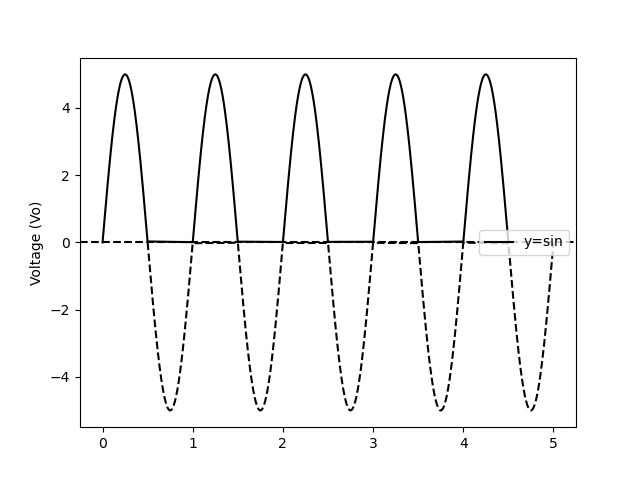
\includegraphics{figs/gate_25_fig5.png}
    \caption{Output Waveform}
    \label{fig:gate_ee_25_5}
\end{figure}

\begin{figure}[H]
    \centering
    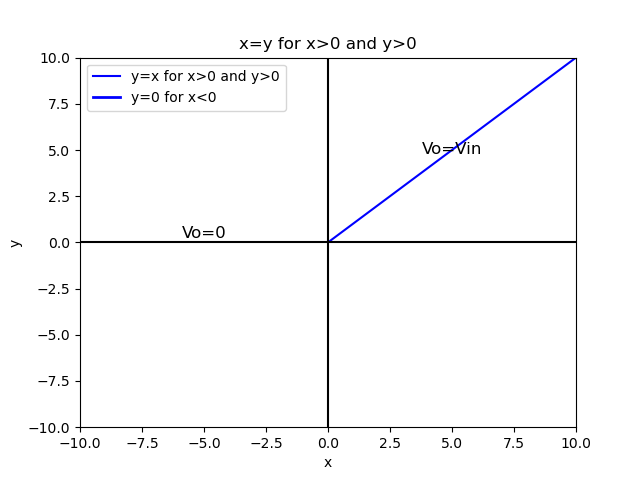
\includegraphics{figs/gate_25_fig6.png}
    \caption{charecterstic graph}
    \label{fig:gate_ee_25_6}
\end{figure}
The solution is Option A
\end{document}


